\chapter{Komplexe Zahlen und Funktionen}
\section{Definition einer komplexen Zahl}
Unter einer komplexen Zahl $z$ versteht man ein geordnetes Paar $(x, y)$ aus zwei reellen Zahlen $x$ und $y$. Symbolische Schreibweise:
$$z=x + jy$$
Die komplexe Zahl $z = x + jy$ wird dabei durch den Punkt $P(z) = (z; y)$ der $x, y$-Ebene eindeutig repräsentiert. Die reellen Bestandteile $x$ und $y$ der komplexen Zahl $z = x+ jy$ werden als Realteil und Imaginärteil von $z$ bezeichnet. Symbolische Schreibweise:
$$Re(z), Im(z)$$
Die Menge $\mathbb{C}=\{z|z=x+jy \text{ mit } x, y \in \mathbb{R}\}$ heisst Menge der komplexen Zahlen.
\subsection{Weitere Grundbegriffe}
\begin{itemize}
	\item Zwei komplexe Zahlen sind genau dann \textbf{gleich}, wenn $Re(z_1) = Re(z_2)$ und $Im(z_1) = Im(z_2)$ gilt.
	\item Der \textbf{Betrag} einer komplexen Zahl ist die Länge des dazugehörigen Zeigers: $|z| = \sqrt{x^2+y^2}$
	\item Der Übergang von der komplexen Zahl $z$ zu \textbf{konjugiert} komplexzen Zahl $z^*$ bedeuted einen Vorzeichenwechsel im Imaginärteil. Der dazugehörige Zeiger liegt daher spiegelsymmetrisch zur reellen Achse. $z^* = (x + jy)^* = x + j(-y) = x - jy$
\end{itemize}

\subsection{Darstellungsformen}
\begin{itemize}
	\item Normalform: $$z=x + jy$$
	\item Trigonometrische Form: $$z= r \cdot (cos\phi + j \cdot sin\phi)$$ 
	\item Exponentialform: $$e^{j\phi} =  cos\phi + j \cdot sin\phi$$ $$ \Rightarrow z = r \cdot (cos\phi + j \cdot sin\phi) = r \cdot e^{j\phi}$$
\end{itemize}
Die trigonometrische Form und die Exponentialform werden auch Polarform genannt.

\subsection{Umrechnung Polarform $\rightarrow$ Kartesische Form}
Eine in der Polarform $z = r (cos\phi + j \cdot sin\phi)$ oder $z=r \cdot e^{j\phi}$ vorliegende komplexe Zahl lässt sich mit Hilfe der Transformationsgleichung 
$$ x = r \cdot cos\phi, y = r \cdot sin\phi$$ 
in die kartesische Form $z = x + jy$ überführen.

\subsection{Umrechnung Kartesische Form $\rightarrow$ Polarform}
eine in der kartesischen Form $z = x + jy$ vorliegende komplexe Zahl lässt sich mit Hilfe der Transformationsgleichungen 
$$ r = |z| = \sqrt{x^2 + y^2}, tan \phi = \frac{y}{x}$$ 
und unter Berüksichtigung des Quadranten, in dem der zugehörige Punkt liegt, in die trigonometrische Form $z = r(cos\phi + j \cdot sin\phi)$ bzw. die Exponentialform $z=e^{j\phi}$ überführen.
\begin{table}[H]
\begin{tabular}{|c|c|c|c|}
\hline 
Quadrant & I & II, III & IV \\ 
\hline 
$\phi =$ & $arctan \frac{y}{x}$ & $arctan \frac{y}{x}+\pi$ & $arctan \frac{y}{x} + 2\pi$ \\ 
\hline 
\end{tabular}
\caption{Tabelle zum Quadranten}
\end{table} 

\begin{figure}[H]
\centering 
	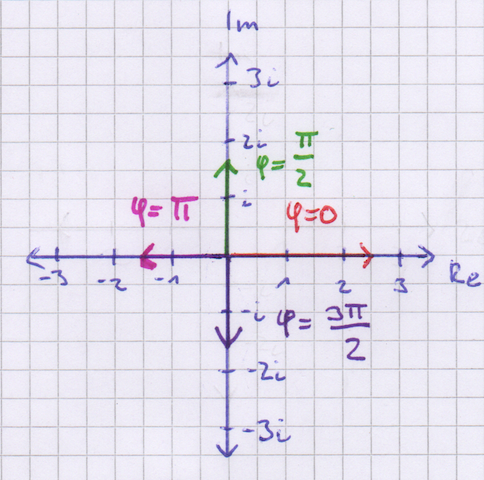
\includegraphics[width=1\textwidth]{Bilder/phi}
\caption{Verhalten von $\phi$}
\end{figure} 


\section{Komplexe Rechnung}
\subsection{Grundrechenarten}
\subsubsection*{Addition und Subtraktion}
\begin{definition}
Summe $z_1 + z_2$ und Differenz $z_1 - z_2$ zweier komplexen Zahlen $z_1 = x_1 + jy_1$ und $z_2 = x_2 + jy_2$ werden nach den folgenden Vorschriften gebildet:
\begin{align*}
z_1 + z_2 &= (x_1 + x_2) + j(y_1 + y_2)\\
z_1 - z_2 &= (x_1 - x_2) + j(y_1 - y_2)\\
\end{align*}
\end{definition}
Bemerkungen:
\begin{itemize}
	\item Realteile und Imaginärteile werden jeweils für sich addiert, bzw. subtrahiert.
	\item Addition und Subtraktion lassen am einfachsten in der kartesischen Form durchführen.
	\item Die Addition ist kummutativ.
	\item Ungleichungen wie $z_1 < z_2$ oder $z_1>z_2$ machen, im Gegensatz zu den reellen Zahlen, keinen Sinn.
\end{itemize}

\subsubsection*{Multiplikation in der kartesischen Form}
\begin{definition}
Das Produkt $z_1 \cdot z_2 = (x_1 + jy_1) \cdot (x_2 + jy_2)$ zweier komplexer Zahlen $z_1$ und $z_2$ wir im Reellen durch "Ausmultiplizieren" der Klammern unter Beachtung der Beziehung $j^2 = -1$ berechnet. Geht am einfachsten in der trigonometrischen Form.
\end{definition}
\begin{bsp}
\begin{align*}
	z_1 \cdot z_2 	&= (x_1 + jy_1)(x_2 + jy_2) \\
							&= x_1x_2 + x_1jy_2 + jy_1x_2 + j^2y_1y_2\\
							&=(x1_x2 - y_1y2) + j(x_1y_2 + x_2y_2)\\
\end{align*}
\end{bsp}
\subsubsection*{Multiplikation in der Polarform}
\begin{definition}
Zwei komplexe Zahlen werden multipliziert, indem man ihre Beträge multipliziert und ihre Argumente (Winkel) addiert.
\begin{align*}
	z_1 \cdot z_2 	&= (r_1r_2)[cos(\phi_1 +\phi_2) +j \cdot sin(\phi_1 + \phi_2)] \\
							&= (r_1r_2) \cdot e^{j(\phi_1 + \phi_2)}
\end{align*}
\end{definition}

\subsubsection*{Division in der kartesischen Form}
\begin{definition}
Der Quotien $z_1/z_2$ zweier komplexen Zahlen $z_1$ und $z_2$ in kartesischer Form lässt sich schrittweise berechnen:
\begin{enumerate}
	\item Der Bruch $z_1/z_2$ wird zunächst mit $z_2^*$, also dem konjugiert komplexen Nenner, erweitert:
	\begin{align*}
	\frac{z_1}{z_2} 	&= \frac{z_1 \cdot z_2^*}{z_2 \cdot z_2^*} &= \frac{(x_1 +jy_1) \cdot (x_2-jy_2)}{(x_2+jy_2)\cdot (x_2-jy_2)}
\end{align*}
	\item Zähler und Nenner werden dann nach den aus dem Rellen bekanten Regeln "ausmultipliziert" ungter Beachtung der Beziehung $j^2 = -1$. Der Nenner des Bruchs wird dadurch (positiv) reell.
	\item Die im Zähler stehende komplexe Zahl wird jetzt gliedweise durch den (reellen) Nenner dividiert.
\end{enumerate}
Man beachte: Wie im Rellen so ist auch im Komplexen die Division durch die Zahl Null nicht erlaubt.
\end{definition}

\subsubsection*{Division in der Polarform}
\begin{definition}
Zwei komplexe Zahlen werden dividiert, indem man ihre Beträge dividiert und ihre Argumente (Winkel) subtrahiert.
\begin{align*}
	\frac{z_1}{z_2} 	&= \frac{r_1}{r_2}[cos(\phi_1 -\phi_2) +j \cdot sin(\phi_1 - \phi_2)] \\
							&= \frac{r_1}{r_2} \cdot e^{j(\phi_1 - \phi_2)}
\end{align*}
\end{definition}

\subsection{Potenzieren und Radizieren}
\begin{definition}
Eine in der Polarform vorliegende komplexe Zahl $z$ wird wie folgt \textbf{potenziert}:
\begin{itemize}
	\item In exponentieller Schreibweise:
	$$ z^n = [r \cdot e^{j\phi}]^n = r^n \cdot e^{jn\phi}$$
	\item In trigonometrischer Schreibweise:
	$$z^n = [r(cos\phi + j \cdot sin \phi)]^n = r^n [cos(n\phi) + j \cdot sin(n\phi)]$$
\end{itemize}
Eine komplexe Zahl wird in die $n$-te Potenz erhoben, in dem man ihren Betrag $r$ in die $n$-te Potenz erhebt und ihr Argument (Winkel $\phi$) mit dem Exponenten $n$ multipliziert. In der Normalform müssen die binomischen Formeln für Potenzen verwendet werden.
\end{definition}

\begin{definition}
Die Gleichung $z^n = a = a_0 \cdot e^{ja}$ $(a_0 > 0; n=1)$ besitzt im Komplexen genau $n$ verschiedene Lösungen (Wurzeln)
$$ z_k = r(cos\phi_k + j \cdot sin\phi_k) = r \cdot e^{j\phi_k}$$
mit
$$ r = \sqrt[n]{a_0} \text{ und } \phi_k = \frac{a + k \cdot 2\phi}{n}$$
($k = 0,1,2,...,n-1$). Die dazugehörigen Bildpunkte liegen in der Gaussschen Zahlenebene auf dem Mittelpunktskreis mit dem Radios $R=\sqrt[n]{a_0}$ und bilden die Ecken eines regelmässigen n-Ecks.
\end{definition}